\documentclass[aspectratio=169,11pt]{beamer}

% ============================================================
% FireForest - Presentacion Avance 1 (Grupo 4)
% Version 2: revision integral (narrativa, metodologia, evidencia
% real, matematica y diseno) sobre la base de la plantilla original
% (Tareas/Proyecto_integrador/15_template_logos/main.tex), recoloreada
% con la paleta ambiente/territorio/fuego usada en el informe
% (avance1_corregido.tex).
% ============================================================

\usepackage[utf8]{inputenc}
\usepackage[T1]{fontenc}
\usepackage{lmodern}
\usepackage[spanish]{babel}
\usepackage{graphicx}
\usepackage{booktabs}
\usepackage{array}
\usepackage{colortbl}
\usepackage{tikz}
\usetikzlibrary{arrows.meta,positioning,calc}
\usepackage{amsmath}

\usetheme{Madrid}
\usecolortheme{default}
\useinnertheme{circles}

% ------------------------------------------------------------
% Paleta ambiente / territorio / fuego (coherente con el informe)
% ------------------------------------------------------------
\definecolor{VerdeOscuro}{RGB}{27,94,55}
\definecolor{VerdeMedio}{RGB}{46,125,80}
\definecolor{VerdePalido}{RGB}{213,234,217}
\definecolor{Tierra}{RGB}{124,89,55}
\definecolor{TierraPalido}{RGB}{237,227,213}
\definecolor{Fuego}{RGB}{196,86,26}
\definecolor{FuegoPalido}{RGB}{250,224,206}
\definecolor{GrisTexto}{RGB}{51,51,51}

\setbeamercolor*{palette primary}{bg=VerdeOscuro, fg=white}
\setbeamercolor*{palette secondary}{bg=VerdeMedio, fg=white}
\setbeamercolor*{palette tertiary}{bg=Tierra, fg=white}
\setbeamercolor*{palette quaternary}{bg=VerdeOscuro, fg=white}
\setbeamercolor{structure}{fg=VerdeOscuro}
\setbeamercolor{section in toc}{fg=VerdeOscuro}
\setbeamercolor{title}{fg=VerdeOscuro}
\setbeamercolor{frametitle}{bg=VerdeOscuro, fg=white}
\setbeamercolor{alerted text}{fg=Fuego}
\setbeamercolor{block title}{bg=VerdeMedio, fg=white}
\setbeamercolor{block body}{bg=VerdePalido, fg=GrisTexto}
\setbeamercolor{block title alerted}{bg=Fuego, fg=white}
\setbeamercolor{block body alerted}{bg=FuegoPalido, fg=GrisTexto}
\setbeamercolor{block title example}{bg=Tierra, fg=white}
\setbeamercolor{block body example}{bg=TierraPalido, fg=GrisTexto}
\setbeamercolor{normal text}{fg=GrisTexto}
\setbeamercolor{item}{fg=VerdeOscuro}

\setbeamertemplate{navigation symbols}{}
\setbeamertemplate{itemize item}{\color{VerdeOscuro}\textbullet}
\setbeamertemplate{itemize subitem}{\color{VerdeMedio}\textendash}
\setbeamerfont{footline}{size=\tiny}

% ------------------------------------------------------------
% Pie de pagina propio: nombre corto FireForest + seccion activa + numeracion
% ------------------------------------------------------------
\newcommand{\seccionactual}{Presentaci\'on}
\setbeamertemplate{footline}{%
  \leavevmode%
  \hbox{%
    \begin{beamercolorbox}[wd=.85\paperwidth,ht=2.6ex,dp=1.2ex,left,leftskip=1em]{author in head/foot}%
      \usebeamerfont{author in head/foot}\tiny FireForest \textbar\ Avance 1 \textbar\ \textbf{\seccionactual} \textbar\ Grupo 4 \textbar\ ESPOCH
    \end{beamercolorbox}%
    \begin{beamercolorbox}[wd=.15\paperwidth,ht=2.6ex,dp=1.2ex,right,rightskip=1em]{date in head/foot}%
      \usebeamerfont{date in head/foot}\tiny \insertframenumber{}/\inserttotalframenumber
    \end{beamercolorbox}%
  }%
}

% ------------------------------------------------------------
% Estilos TikZ reutilizados
% ------------------------------------------------------------
\tikzset{
  flowbox/.style={draw=VerdeOscuro, rounded corners, fill=VerdePalido,
    align=center, text width=#1, minimum height=0.8cm, font=\footnotesize, inner sep=3pt},
  flowbox/.default=3.1cm,
  flowarr/.style={-{Latex[length=2.9mm, width=2.1mm]}, line width=1.1pt, VerdeOscuro},
  zonebox/.style={draw=Tierra, rounded corners, fill=TierraPalido,
    align=center, text width=3.0cm, minimum height=1.6cm, font=\footnotesize, inner sep=3pt},
  warnbox/.style={draw=Fuego, rounded corners, thick, fill=FuegoPalido,
    align=center, text width=#1, font=\footnotesize, inner sep=5pt},
  warnbox/.default=10cm,
  argbox/.style={draw=VerdeOscuro, rounded corners, thick, fill=VerdePalido,
    align=center, text width=#1, font=\footnotesize, inner sep=6pt},
  argbox/.default=10cm,
  smallflow/.style={draw=Tierra, rounded corners, fill=TierraPalido,
    align=center, text width=2.35cm, minimum height=1.15cm, font=\scriptsize, inner sep=3pt},
  % ---- estilos de arquitectura reutilizados en las diapositivas 6 y 14 ----
  origenbox/.style={draw=Tierra, line width=1pt, rounded corners, fill=TierraPalido,
    align=center, text width=#1, minimum height=0.6cm, font=\footnotesize, inner sep=3pt},
  origenbox/.default=11.8cm,
  procesobox/.style={draw=VerdeOscuro, line width=1pt, rounded corners, fill=VerdePalido,
    align=center, text width=#1, minimum height=0.5cm, font=\footnotesize, inner sep=3pt},
  procesobox/.default=11.8cm,
  docbox/.style={draw=Tierra, line width=1.1pt, rounded corners, fill=TierraPalido,
    align=center, text width=#1, minimum height=0.55cm, font=\footnotesize, inner sep=3pt},
  docbox/.default=5.5cm,
  relbox/.style={draw=VerdeOscuro, line width=1.1pt, rounded corners, fill=VerdePalido,
    align=center, text width=#1, minimum height=0.55cm, font=\footnotesize, inner sep=3pt},
  relbox/.default=5.5cm,
  prodbox/.style={draw=Fuego, line width=1.1pt, rounded corners, fill=FuegoPalido,
    align=center, text width=#1, minimum height=0.5cm, font=\footnotesize\bfseries, inner sep=3pt},
  prodbox/.default=11.8cm,
  ctrlbox/.style={draw=VerdeMedio, line width=1pt, rounded corners, fill=VerdeMedio!18,
    align=center, text width=#1, font=\tiny, inner sep=4pt},
  ctrlbox/.default=11.8cm,
  microflow/.style={draw=VerdeOscuro, line width=0.9pt, rounded corners, fill=VerdePalido,
    align=center, text width=#1, minimum height=0.5cm, font=\tiny, inner sep=2pt},
  microflow/.default=2.3cm,
  airbox/.style={draw=Tierra, line width=0.9pt, dashed, rounded corners, fill=TierraPalido!35,
    align=center, text width=#1, font=\tiny, inner sep=4pt},
  airbox/.default=11.8cm,
  stepnum/.style={circle, draw=VerdeOscuro, line width=0.8pt, fill=white,
    text=VerdeOscuro, font=\tiny\bfseries, minimum size=0.36cm, inner sep=0pt},
}

% Comando para linea de fuente al pie de una diapositiva
\newcommand{\fuente}[1]{{\vfill\tiny\color{GrisTexto!70!black} Fuente: #1}}

% ------------------------------------------------------------
% Metadatos
% ------------------------------------------------------------
\title[FireForest -- Avance 1]{Dise\~no de una arquitectura h\'ibrida SQL--NoSQL para la integraci\'on y consulta de datos de incendios forestales en el cant\'on Loja}
\author[Malan, Pujos, Chuncho]{Malan Mullo, Marco Vinicio \and Pujos Culque, Viviana Isabel \and Chuncho Morocho, Carlos Guillermo}
\institute[ESPOCH]{Escuela Superior Polit\'ecnica de Chimborazo (ESPOCH)\\ Maestr\'ia en Estad\'istica con menci\'on en Ciencia de Datos e Inteligencia Artificial}
\date{Avance 1 \textbar\ 2026}

\begin{document}

% ============================================================
% 1 - PORTADA
% ============================================================
{\setbeamertemplate{footline}{}
\begin{frame}[plain]
  \centering
  \begin{columns}[c]
    \column{0.5\textwidth}
      \centering
\includegraphics[height=1.25cm]{logos/logo_espoch.png}
    \column{0.5\textwidth}
      \centering
\includegraphics[height=1.25cm]{logos/logo_maestria.jpeg}
  \end{columns}

  \vspace{0.25cm}
  {\footnotesize ESCUELA SUPERIOR POLIT\'ECNICA DE CHIMBORAZO (ESPOCH)\par}
  {\scriptsize Maestr\'ia en Estad\'istica con menci\'on en Ciencia de Datos e Inteligencia Artificial\par}

  \vspace{0.3cm}
  {\color{VerdeOscuro}\rule{0.75\textwidth}{0.6pt}\par}
  \vspace{0.22cm}
  \begin{minipage}{0.85\textwidth}
  \centering{\large\bfseries\color{VerdeOscuro} Dise\~no de una arquitectura h\'ibrida SQL--NoSQL para la integraci\'on y consulta de datos de incendios forestales en el cant\'on Loja\par}
  \end{minipage}
  \vspace{0.22cm}
  {\color{VerdeOscuro}\rule{0.75\textwidth}{0.6pt}\par}

  \vspace{0.3cm}
  {\small
  Malan Mullo, Marco Vinicio\\
  Pujos Culque, Viviana Isabel\\
  Chuncho Morocho, Carlos Guillermo\par}

  \vspace{0.25cm}
  {\small\bfseries\color{Tierra} Grupo 4\par}
  \vspace{0.12cm}
  {\small Avance 1 \textbar\ 2026\par}
\end{frame}
}

% ============================================================
% 2 - RUTA DE LA EXPOSICION
% ============================================================
\begin{frame}{Ruta de la exposici\'on}
  \vspace{0.2cm}
  \begin{center}
  \begin{tikzpicture}[
    ag/.style={draw=VerdeOscuro, rounded corners, fill=VerdePalido, minimum width=10.5cm,
      minimum height=1.0cm, align=left, font=\normalsize, inner sep=8pt},
    num/.style={circle, draw=white, fill=VerdeOscuro, text=white, font=\bfseries, minimum size=0.72cm}
  ]
    \node[ag] (a1) {\phantom{X}\hspace{0.9cm} Introducci\'on};
    \node[num] at ([xshift=0.65cm]a1.west) {1};
    \node[ag, below=0.22cm of a1] (a2) {\phantom{X}\hspace{0.9cm} Metodolog\'ia};
    \node[num] at ([xshift=0.65cm]a2.west) {2};
    \node[ag, below=0.22cm of a2] (a3) {\phantom{X}\hspace{0.9cm} Resultados preliminares};
    \node[num] at ([xshift=0.65cm]a3.west) {3};
    \node[ag, below=0.22cm of a3] (a4) {\phantom{X}\hspace{0.9cm} Discusi\'on preliminar};
    \node[num] at ([xshift=0.65cm]a4.west) {4};
    \node[ag, below=0.22cm of a4] (a5) {\phantom{X}\hspace{0.9cm} Conclusiones y pr\'oximos pasos};
    \node[num] at ([xshift=0.65cm]a5.west) {5};
  \end{tikzpicture}
  \end{center}
\end{frame}

\renewcommand{\seccionactual}{I. Introducci\'on}
% ============================================================
% 3 - INTRODUCCION: CONTEXTO TERRITORIAL Y AMBIENTAL
% ============================================================
\begin{frame}{Introducci\'on: contexto territorial y ambiental}
  \begin{columns}[T]
    \column{0.54\textwidth}
      \scriptsize
      \begin{itemize}\itemsep0pt\parskip1pt
        \item El cant\'on Loja se ubica en los \textbf{Andes tropicales} del sur de Ecuador.
        \item El relieve monta\~noso genera \textbf{transiciones ambientales pronunciadas}.
        \item Temperatura, precipitaci\'on, humedad, vegetaci\'on y combustibles cambian con la altitud.
        \item Condiciones contrastantes entre \textbf{Malacatos, Punzara y San Lucas}.
        \item El estudio de referencia abarca \textbf{$\sim$1549--2757 m s.\,n.\,m.}
      \end{itemize}
      \vspace{0.06cm}
      {\scriptsize\color{Tierra}\textbf{Estas diferencias modifican los controles ambientales del comportamiento del fuego.}}
    \column{0.42\textwidth}
      \centering
      \begin{tikzpicture}[
        zn/.style={draw=Tierra, rounded corners, fill=TierraPalido, align=center,
          text width=2.1cm, minimum height=0.62cm, font=\scriptsize, inner sep=2pt}
      ]
        \node[zn] (sl) {San Lucas\\ $\sim$2752--2757 m};
        \node[zn, below=0.15cm of sl] (pz) {Punzara\\ $\sim$2270--2278 m};
        \node[zn, below=0.15cm of pz] (mc) {Malacatos\\ $\sim$1549--1557 m};
        \node[draw=VerdeOscuro, rounded corners, fill=VerdePalido, align=center,
          minimum width=2.1cm, minimum height=0.8cm, font=\scriptsize\bfseries,
          right=0.5cm of pz] (loja) {Cant\'on\\ Loja};
        \draw[flowarr] (sl) -- (loja);
        \draw[flowarr] (pz) -- (loja);
        \draw[flowarr] (mc) -- (loja);
      \end{tikzpicture}
  \end{columns}

  \vspace{0.2cm}
  \begin{columns}[T]
    \column{0.36\textwidth}
      \centering
      
\includegraphics[width=4.2cm]{figuras/articulo_fire_ecology_recortado.png}
    \column{0.64\textwidth}
      \vspace{0.04cm}
      {\scriptsize Estudio de referencia desarrollado en Malacatos, Punzara y San Lucas, utilizado para contextualizar la heterogeneidad ambiental y altitudinal del cant\'on Loja.\par}
      \vspace{0.05cm}
      {\scriptsize Balaguer-Beser et al. (2026). DOI: \href{https://doi.org/10.1186/s42408-026-00470-y}{10.1186/s42408-026-00470-y}\par}
  \end{columns}
  \fuente{elaboraci\'on propia con base en Balaguer-Beser et al. (2026); resultados v\'alidos para las 3 zonas de estudio, no generalizables a todo el cant\'on.}
\end{frame}

% ============================================================
% 4 - INTRODUCCION: PROBLEMA Y BRECHA
% ============================================================
\begin{frame}{Introducci\'on: problema y brecha}
  \begin{center}
  \begin{tikzpicture}
    \node[argbox=11.4cm] (arg) {\footnotesize La heterogeneidad territorial y ambiental de Loja condiciona el an\'alisis del comportamiento del fuego. Para estudiarla deben integrarse observaciones espaciales, clim\'aticas y satelitales que difieren en formato, resoluci\'on y granularidad. La carencia de un flujo integrado, trazable y reproducible constituye la brecha de Ingenier\'ia de Datos abordada por FireForest.};
  \end{tikzpicture}
  \end{center}
  \vspace{0.5cm}
  \begin{center}
  \begin{tikzpicture}
    \node[smallflow] (b1) {Heterogeneidad ambiental};
    \node[smallflow, right=0.5cm of b1] (b2) {Datos heterog\'eneos};
    \node[smallflow, right=0.5cm of b2] (b3) {Dificultad de integraci\'on};
    \node[smallflow, right=0.5cm of b3] (b4) {Brecha reproducible};
    \draw[flowarr] (b1) -- (b2);
    \draw[flowarr] (b2) -- (b3);
    \draw[flowarr] (b3) -- (b4);
  \end{tikzpicture}
  \end{center}
  \fuente{Balaguer-Beser et al. (2026) y elaboraci\'on propia.}
\end{frame}

% ============================================================
% 5 - PREGUNTA, OBJETIVO Y ALCANCE
% ============================================================
\begin{frame}{Pregunta, objetivo y alcance}
  \begin{center}
  \begin{tikzpicture}
    \node[argbox=11.8cm, inner sep=3pt] (preg) {\footnotesize \textbf{Pregunta principal (arquitectura):} \textquestiondown C\'omo dise\~nar una arquitectura h\'ibrida SQL--NoSQL que permita integrar, almacenar y consultar de forma reproducible datos heterog\'eneos de incendios forestales en Loja?};
  \end{tikzpicture}
  \end{center}
  \vspace{0.05cm}
  \begin{center}
  \begin{tikzpicture}
    \node[draw=Tierra, very thick, rounded corners, fill=TierraPalido,
      text width=11.8cm, align=center, font=\footnotesize, inner sep=3pt] (obj)
      {\textbf{Objetivo general:} dise\~nar una arquitectura h\'ibrida SQL--NoSQL para integrar VIIRS, CHIRPS y una malla espacial de Loja, construyendo un dataset anal\'itico reproducible por celda y mes.};
  \end{tikzpicture}
  \end{center}
  \vspace{0.05cm}
  {\scriptsize\color{GrisTexto!70!black}\textbf{Pregunta anal\'itica futura (no respondida en este avance):} \textquestiondown existe relaci\'on entre la precipitaci\'on mensual y la ocurrencia de \textbf{detecciones} de incendio por celda? \textit{(VIIRS aporta detecciones, no un conteo de incendios independientes.)}\par}
  \vspace{0.06cm}
  \begin{columns}[T]
    \column{0.47\textwidth}
      \textbf{\scriptsize\color{VerdeOscuro}Incluye este Avance 1}
      \begin{itemize}\scriptsize\itemsep0pt\parskip0pt
        \item Arquitectura h\'ibrida y modelos SQL/NoSQL
        \item Datos controlados y consultas iniciales
        \item Validaciones preliminares reproducibles
      \end{itemize}
    \column{0.06\textwidth}
      \phantom{x}
    \column{0.47\textwidth}
      \textbf{\scriptsize\color{Fuego}Todav\'ia no incluye}
      \begin{itemize}\scriptsize\itemsep0pt\parskip0pt
        \item Sistema operativo ni alerta temprana
        \item Datos reales completos ni modelo predictivo
        \item Relaci\'on causal clima--incendio
      \end{itemize}
  \end{columns}
  \vspace{0.05cm}
  \begin{center}
  \begin{tikzpicture}
    \node[warnbox=11.8cm, inner sep=3pt] {\footnotesize \textbf{Dominio previsto:} cant\'on Loja. \textbf{Cobertura actual del prototipo:} dos celdas controladas utilizadas exclusivamente para validar el flujo de datos; no representan el territorio cantonal.};
  \end{tikzpicture}
  \end{center}
\end{frame}

\renewcommand{\seccionactual}{II. Metodolog\'ia}
% ============================================================
% 6 - ARQUITECTURA GENERAL DEL SISTEMA
% ============================================================
\begin{frame}{Arquitectura general del sistema}
  \centering
  \begin{tikzpicture}
    \node[origenbox] (fuentes) {\textbf{Fuentes originales} \\ \tiny NASA FIRMS \textbar\ CHIRPS \textbar\ l\'imite espacial institucional (pendiente)};
    \node[procesobox, below=0.2cm of fuentes] (adq) {\textbf{Adquisici\'on e ingesta} \\ \tiny API o descarga directa \textbar\ lectura de archivos \textbar\ validaci\'on inicial};
    \node[procesobox, below=0.2cm of adq] (val) {\textbf{Validaci\'on y transformaci\'on} \\ \tiny estructura \textbar\ fechas \textbar\ coordenadas \textbar\ calidad \textbar\ duplicados};
    \node[docbox, below=0.4cm of val, xshift=-3.25cm] (mongo) {\textbf{MongoDB} \\ \tiny Detecciones individuales y metadatos};
    \node[relbox, below=0.4cm of val, xshift=3.25cm] (pg) {\textbf{PostgreSQL / PostGIS} \\ \tiny Celdas, calendario, clima y agregados diarios};
    \node[procesobox] (integra) at ($(mongo.south)!0.5!(pg.south) + (0,-0.42cm)$) {\textbf{Integraci\'on} \\ \tiny Uni\'on l\'ogica por \texttt{celda\_id} y fecha};
    \node[prodbox, below=0.2cm of integra] (dataset) {Dataset anal\'itico celda-mes};
    \draw[flowarr] (fuentes) -- (adq);
    \draw[flowarr] (adq) -- (val);
    \draw[flowarr] (val.south) -- (mongo.north);
    \draw[flowarr] (val.south) -- (pg.north);
    \draw[flowarr] (mongo.south) -- (integra.north);
    \draw[flowarr] (pg.south) -- (integra.north);
    \draw[flowarr] (integra) -- (dataset);
    \node[stepnum] at ([xshift=-0.22cm]fuentes.west) {1};
    \node[stepnum] at ([xshift=-0.22cm]adq.west) {2};
    \node[stepnum] at ([xshift=-0.22cm]val.west) {3};
    \node[stepnum] at ([xshift=-0.22cm]mongo.west) {4};
    \node[stepnum] at ([xshift=-0.22cm]integra.west) {5};
    \node[stepnum] at ([xshift=-0.22cm]dataset.west) {6};
  \end{tikzpicture}

  \vspace{0.15cm}
  {\footnotesize\color{GrisTexto!70!black} M\'etodo previsto de adquisici\'on: API o descarga directa de NASA FIRMS y repositorio CHIRPS. El prototipo actual utiliza datos controlados cargados desde archivos locales.\par}
  \fuente{elaboraci\'on propia.}
\end{frame}

% ============================================================
% 7 - IMPLEMENTACION LOCAL Y COLABORACION MEDIANTE GITHUB
% ============================================================
\begin{frame}{Implementaci\'on local y colaboraci\'on mediante GitHub}
  \begin{columns}[T]
    \column{0.475\textwidth}
      \centering
      {\scriptsize\bfseries\color{VerdeOscuro} Entorno local en VS Code\par}
      \vspace{0.06cm}
      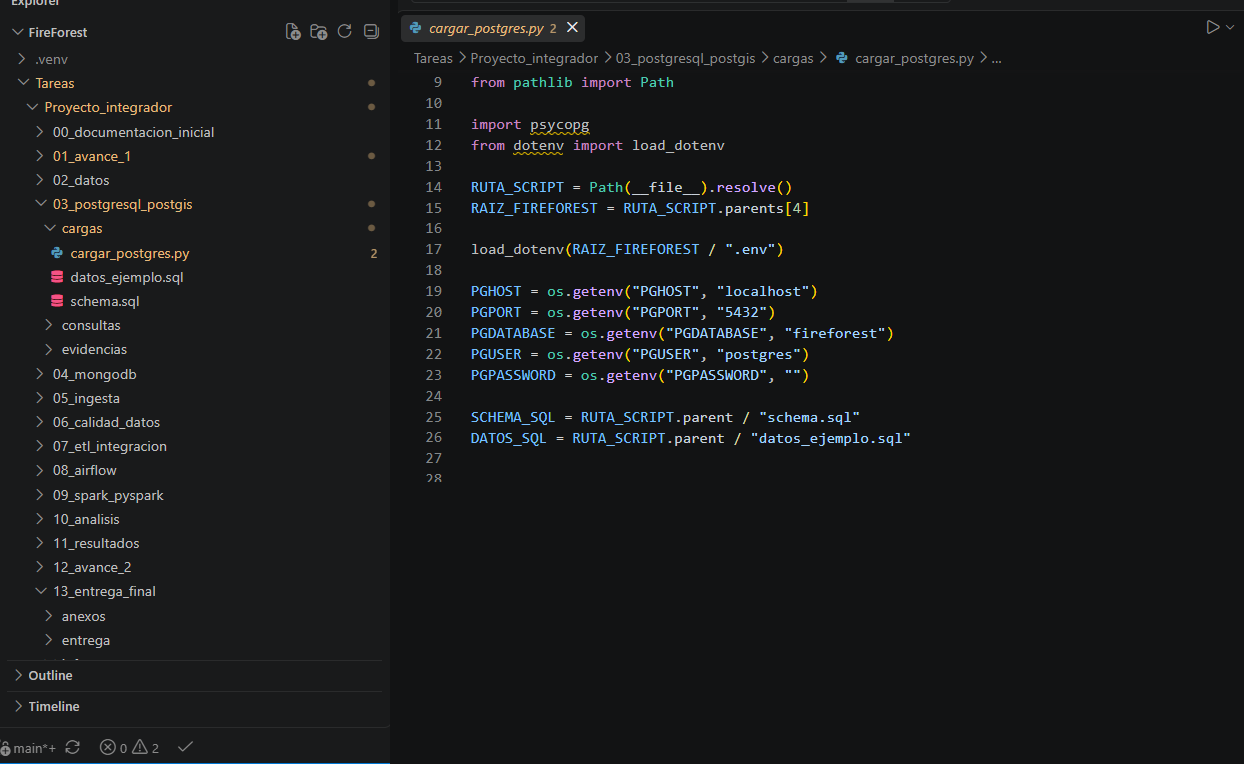
\includegraphics[width=\linewidth]{figuras/captura_vscode_recortada.png}
      \vspace{0.08cm}

      {\tiny La estructura local organiza los m\'odulos t\'ecnicos del proyecto y permite desarrollar y ejecutar los scripts de carga, consulta y validaci\'on.\par}
    \column{0.05\textwidth}
      \phantom{x}
    \column{0.475\textwidth}
      \centering
      {\scriptsize\bfseries\color{VerdeOscuro} Repositorio remoto en GitHub\par}
      \vspace{0.06cm}
      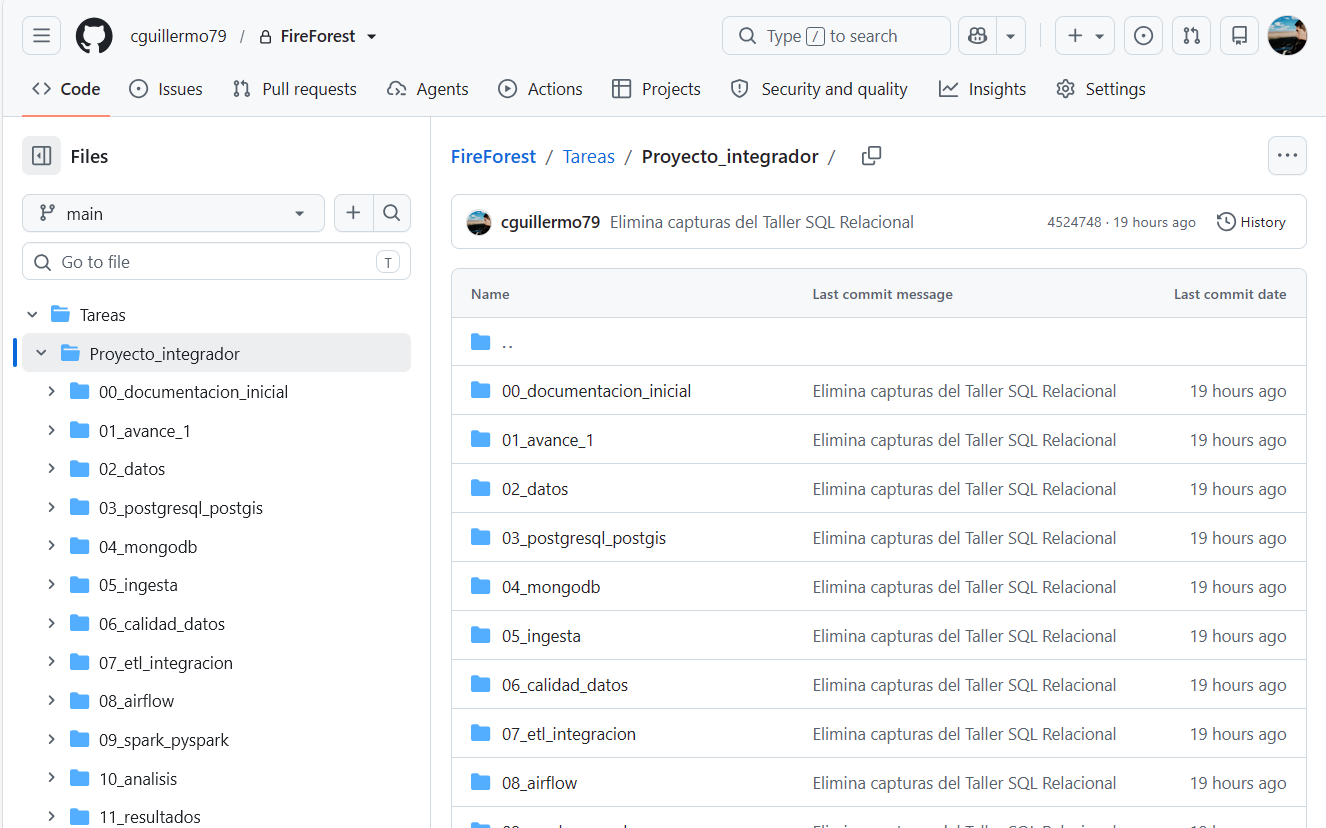
\includegraphics[width=\linewidth]{figuras/captura_github_recortada.png}
      \vspace{0.08cm}

      {\tiny El repositorio remoto centraliza el c\'odigo y la documentaci\'on de FireForest, facilita el intercambio de avances y permite mantener el control de versiones del trabajo del grupo.\par}
  \end{columns}
  \fuente{capturas propias de los entornos de desarrollo local y remoto de FireForest, 2026.}
\end{frame}

% ============================================================
% 8 - FUENTES Y VARIABLES
% ============================================================
\begin{frame}{Fuentes y variables}
  \raggedright{\small\textbf{Tabla 1. Fuentes, variables y transformaciones del proyecto}\par}
  \vspace{0.05cm}
  \begin{center}
  \tiny
  \setlength{\tabcolsep}{2.8pt}
  \begin{tabular}{@{}p{1.15cm}p{1.55cm}p{2.35cm}p{1.55cm}p{2.7cm}p{2.35cm}@{}}
  \toprule
  \textbf{Fuente} & \textbf{Var. original} & \textbf{Significado / unidad} & \textbf{Resoluci\'on} & \textbf{Transformaci\'on} & \textbf{Variable final} \\
  \midrule
  VIIRS & \texttt{frp\_mw} & Potencia radiativa, MW & Detecci\'on & Agregaci\'on diaria y mensual & \texttt{frp\_suma\_mw}; \texttt{frp\_maxima\_mw} \\
  VIIRS & \texttt{coordenadas} & Ubicaci\'on de la detecci\'on & Punto & Asignaci\'on espacial a celda & \texttt{celda\_id} \\
  CHIRPS & precipitaci\'on & Precipitaci\'on diaria, mm & P\'ixel-d\'ia, $\sim$0.05\textdegree & Asignaci\'on y agregaci\'on mensual & \texttt{precipitacion\_\allowbreak acumulada\_\allowbreak mensual\_mm} \\
  Malla & long./lat. & Ubicaci\'on de la celda & Punto (4326) & \texttt{ST\_SetSRID} + \texttt{ST\_Transform} + \texttt{ST\_MakeEnvelope} & \texttt{geom} (32717); \texttt{area\_km2} \\
  Calendario & \texttt{fecha} & D\'ia de observaci\'on & D\'ia & Derivar a\~no y mes & \texttt{fecha\_id}; \texttt{anio}; \texttt{mes} \\
  \bottomrule
  \end{tabular}
  \end{center}
  \vspace{0.2cm}
  {\scriptsize\begin{itemize}\scriptsize
    \item \textbf{Fuente original y acceso:} VIIRS es distribuido por NASA FIRMS (API/descarga directa por \'area y periodo); CHIRPS v2.0 se descarga directamente del repositorio del Climate Hazards Center. La arquitectura no utiliza Google Earth Engine.
    \item Nombres adaptados exactamente a \texttt{schema.sql} y a la consulta corregida; \textbf{malla = 2 celdas controladas}, fuente institucional definitiva pendiente.
    \item Producto VIIRS definitivo y campo de calidad (\texttt{fire\_mask} vs.\ \texttt{confidence}) \textbf{pendientes} de confirmar.
    \item CHIRPS v2.0 ($\sim$5 km nativo) asignada a la malla de 500 m: \textbf{no mejora} su resoluci\'on real.
  \end{itemize}}
  \fuente{NASA FIRMS (VIIRS); Climate Hazards Center (CHIRPS v2.0); \texttt{schema.sql} y \texttt{consulta\_01\_incendios\_clima\_mensual.sql} (elaboraci\'on propia).}
\end{frame}

% ============================================================
% 9 - UNIDAD DE ANALISIS Y GRANULARIDAD
% ============================================================
\begin{frame}{Unidad de an\'alisis y granularidad}
  \begin{center}
  \begin{tikzpicture}
    \node[flowbox=3.3cm] (g1) {Detecci\'on individual\\ \scriptsize (MongoDB, celda\_id+fecha exacta)};
    \node[flowbox=3.1cm, right=0.6cm of g1] (g2) {Celda-d\'ia\\ \scriptsize (\texttt{fact\_incendio} / \texttt{fact\_clima}, PostgreSQL)};
    \node[flowbox=3.1cm, right=0.6cm of g2] (g3) {Celda-mes\\ \scriptsize (dataset anal\'itico, \texttt{GROUP BY})};
    \draw[flowarr] (g1) -- (g2);
    \draw[flowarr] (g2) -- (g3);
  \end{tikzpicture}
  \end{center}
  \vspace{0.35cm}
  \textbf{\small \textquestiondown Por qu\'e no son equivalentes?}
  \begin{itemize}\small
    \item La detecci\'on individual conserva hora exacta y puede haber varias por celda-d\'ia; se pierde ese detalle al agregar.
    \item \texttt{fact\_incendio}/\texttt{fact\_clima} son \textbf{siempre diarios} (\texttt{UNIQUE(celda\_id, fecha\_id)}); nunca existe una fila pre-agregada por mes en las tablas base.
    \item El agregado mensual (\texttt{GROUP BY anio, mes}) puede ocultar variaci\'on diaria real dentro del mes.
  \end{itemize}
  \fuente{elaboraci\'on propia, con base en \texttt{diseno\_sql\_nosql.md} (secci\'on ``Unidad de an\'alisis'').}
\end{frame}

% ============================================================
% 10 - MODELO RELACIONAL
% ============================================================
\begin{frame}{Modelo relacional}
  \raggedright{\small\textbf{Tabla 2. Estructura del modelo relacional}\par}
  \vspace{0.05cm}
  \small
  \begin{center}
  \setlength{\tabcolsep}{3pt}
  \begin{tabular}{@{}p{2.55cm}p{2.5cm}p{3.5cm}p{2.9cm}@{}}
  \toprule
  \textbf{Tabla} & \textbf{Funci\'on} & \textbf{Una fila representa} & \textbf{Clave / v\'inculo} \\
  \midrule
  \texttt{dim\_celda} & Cat\'alogo espacial & Una celda controlada de 500$\times$500 m & \texttt{celda\_id} (PK) \\
  \texttt{dim\_fecha} & Calendario & Un d\'ia & \texttt{fecha\_id} (PK) \\
  \texttt{fact\_incendio} & Detecciones diarias agregadas & Una celda en un d\'ia & \texttt{celda\_id} + \texttt{fecha\_id} (UNIQUE); FK a ambas dimensiones \\
  \texttt{fact\_clima} & Precipitaci\'on diaria & Una celda en un d\'ia & \texttt{celda\_id} + \texttt{fecha\_id} (UNIQUE); FK a ambas dimensiones \\
  \bottomrule
  \end{tabular}
  \end{center}
  \vspace{0.05cm}
  {\small \texttt{fact\_incendio} y \texttt{fact\_clima} \textbf{no} tienen FK entre s\'i: se cruzan mediante \texttt{JOIN} por \texttt{celda\_id} + \texttt{fecha\_id} cuando se necesita comparar incendio y clima.}
  \fuente{\texttt{03\_postgresql\_postgis/cargas/schema.sql}.}
\end{frame}

% ============================================================
% 11 - MODELO DOCUMENTAL
% ============================================================
\begin{frame}[fragile]{Modelo documental}
  \begin{columns}[T]
    \column{0.5\textwidth}
      \begin{footnotesize}
      \begin{verbatim}
{
 "deteccion_id": "V_2023_0001",
 "celda_id": "LJ_04521",
 "fecha": "2023-08-15",
 "frp_mw": 18.4,
 "fire_mask": 7,
 "coordenadas": {
   "longitud": -79.241,
   "latitud": -4.082
 },
 "calidad": { "valida": true }
}
      \end{verbatim}
      \end{footnotesize}
    \column{0.5\textwidth}
      \begin{itemize}\small
        \item \texttt{coordenadas} y \texttt{calidad} son objetos \textbf{anidados}: pueden ganar o perder campos entre versiones del producto VIIRS sin romper el esquema.
        \item El v\'inculo con \texttt{celda\_id} es \textbf{l\'ogico}, no una FK f\'isica: MongoDB no referencia tablas de PostgreSQL.
        \item El prototipo filtra los documentos mediante \texttt{calidad.valida=true} y conserva \texttt{fire\_mask} como atributo de la detecci\'on. El producto VIIRS y el criterio definitivo de calidad deber\'an confirmarse antes de utilizar datos reales.
      \end{itemize}
  \end{columns}
  \fuente{\texttt{04\_mongodb/cargas/detecciones\_viirs.json} (documento real); v\'inculo l\'ogico documentado en \texttt{diseno\_sql\_nosql.md}.}
\end{frame}

% ============================================================
% 12 - ESTANDARIZACION ESPACIAL
% ============================================================
\begin{frame}{Estandarizaci\'on espacial}
  \begin{columns}[T]
    \column{0.5\textwidth}
      \footnotesize
      \begin{align*}
        (x_i, y_i) &= T_{4326\to32717}(\lambda_i, \varphi_i) \\[-2pt]
        C_i &= [x_i{-}250, x_i{+}250]\times[y_i{-}250, y_i{+}250] \\[-2pt]
        A(C_i) &= 500\,\text{m}\times500\,\text{m} = 250\,000\,\text{m}^2
      \end{align*}
    \column{0.5\textwidth}
      \vspace{0.15cm}
      {\tiny $i$ = celda; $(\lambda_i,\varphi_i)$ = longitud/latitud en EPSG:4326.\\[2pt]
      $(x_i,y_i)$ = punto reproyectado en EPSG:32717 (metros).\\[2pt]
      $C_i$ = celda cuadrada de 500 m centrada en $(x_i,y_i)$.\par}
  \end{columns}
  \centering

  \vspace{0.1cm}
  \begin{tikzpicture}[yscale=1, every node/.style={font=\tiny}]
    \node[microflow=2.6cm] (v1) {\textbf{VIIRS}\\ Punto en EPSG:4326};
    \node[microflow=2.4cm, right=0.28cm of v1] (v2) {Reproyecci\'on};
    \node[microflow=2.6cm, right=0.28cm of v2] (v3) {Asignaci\'on espacial};
    \node[microflow=2.2cm, right=0.28cm of v3] (v4) {\texttt{celda\_id}};
    \draw[flowarr] (v1) -- (v2);
    \draw[flowarr] (v2) -- (v3);
    \draw[flowarr] (v3) -- (v4);

    \node[microflow=2.6cm, below=0.22cm of v1] (m1) {\textbf{Malla}\\ Centro o l\'imite espacial};
    \node[microflow=2.4cm, right=0.28cm of m1] (m2) {EPSG:32717};
    \node[microflow=2.6cm, right=0.28cm of m2] (m3) {Pol\'igono 500$\times$500 m};
    \node[microflow=2.2cm, right=0.28cm of m3] (m4) {\texttt{dim\_celda.geom}};
    \draw[flowarr] (m1) -- (m2);
    \draw[flowarr] (m2) -- (m3);
    \draw[flowarr] (m3) -- (m4);

    \node[microflow=2.6cm, below=0.22cm of m1] (c1) {\textbf{CHIRPS}\\ P\'ixel $\sim$0,05\textdegree};
    \node[microflow=2.4cm, right=0.28cm of c1] (c2) {Superposici\'on espacial};
    \node[microflow=2.6cm, right=0.28cm of c2] (c3) {Asignaci\'on a celdas};
    \node[microflow=2.2cm, right=0.28cm of c3] (c4) {Precipitaci\'on por celda};
    \draw[flowarr] (c1) -- (c2);
    \draw[flowarr] (c2) -- (c3);
    \draw[flowarr] (c3) -- (c4);
  \end{tikzpicture}

  \vspace{0.18cm}
  {\footnotesize\color{VerdeOscuro}\textbf{La estandarizaci\'on espacial lleva detecciones, celdas y precipitaci\'on a una referencia com\'un basada en \texttt{celda\_id}. La asignaci\'on de CHIRPS a celdas de 500 m no aumenta su resoluci\'on espacial.}\par}
  \fuente{elaboraci\'on propia (procedimiento); funciones documentadas en PostGIS Documentation.}
\end{frame}

% ============================================================
% 13 - ESTANDARIZACION TEMPORAL
% ============================================================
\begin{frame}{Estandarizaci\'on temporal}
  \begin{columns}[T]
    \column{0.46\textwidth}
      \tiny
      \begin{align*}
        N_{i,m} &= \sum_{d \in m} N_{i,d} \\[-7pt]
        \mathrm{FRP}^{\mathrm{suma}}_{i,m} &= \sum_{d \in m} \mathrm{FRP}_{i,d} \\[-7pt]
        \mathrm{FRP}^{\max}_{i,m} &= \max_{d \in m}\bigl(\mathrm{FRP}^{\max}_{i,d}\bigr) \\[-7pt]
        P_{i,m} &= \sum_{d \in m} P_{i,d}
      \end{align*}
    \column{0.54\textwidth}
      \vspace{0.04cm}
      {\tiny $i$: celda espacial. \quad $d$: d\'ia. \quad $m$: mes.\\[1pt]
      $N_{i,d}$: n\'umero de detecciones en la celda $i$ durante el d\'ia $d$.\\[1pt]
      $\mathrm{FRP}_{i,d}$: potencia radiativa acumulada en la celda y d\'ia.\\[1pt]
      $\mathrm{FRP}^{\max}_{i,d}$: m\'axima potencia radiativa diaria.\\[1pt]
      $P_{i,d}$: precipitaci\'on diaria asignada a la celda.\par}
  \end{columns}

  \vspace{0.08cm}
  \centering
  \begin{tikzpicture}[every node/.style={font=\tiny}]
    \node[microflow=2.3cm] (v1) {\textbf{VIIRS}\\ Detecci\'on individual\\ fecha y hora};
    \node[microflow=1.6cm, right=0.12cm of v1] (v2) {Agrupaci\'on por\\ celda y d\'ia};
    \node[microflow=1.65cm, right=0.12cm of v2] (v3) {\texttt{fact\_incendio}\\ celda-d\'ia};
    \node[microflow=1.5cm, right=0.12cm of v3] (v4) {Agregaci\'on\\ mensual};
    \node[microflow=1.65cm, right=0.12cm of v4] (v5) {Detecciones\\ y FRP};
    \draw[flowarr] (v1) -- (v2);
    \draw[flowarr] (v2) -- (v3);
    \draw[flowarr] (v3) -- (v4);
    \draw[flowarr] (v4) -- (v5);

    \node[microflow=2.3cm, below=0.3cm of v1] (c1) {\textbf{CHIRPS}\\ Precipitaci\'on\\ p\'ixel-d\'ia};
    \node[microflow=1.6cm, right=0.12cm of c1] (c2) {Asignaci\'on\\ a celda};
    \node[microflow=1.65cm, right=0.12cm of c2] (c3) {\texttt{fact\_clima}\\ celda-d\'ia};
    \node[microflow=1.5cm, right=0.12cm of c3] (c4) {Suma\\ mensual};
    \node[microflow=1.65cm, right=0.12cm of c4] (c5) {Precipitaci\'on\\ acumulada};
    \draw[flowarr] (c1) -- (c2);
    \draw[flowarr] (c2) -- (c3);
    \draw[flowarr] (c3) -- (c4);
    \draw[flowarr] (c4) -- (c5);

    \node[prodbox=2.05cm, minimum height=1.35cm, font=\tiny\bfseries, anchor=west]
      (dataset) at ($(v5.east)!0.5!(c5.east) + (0.24cm,0)$) {Dataset\\ anal\'itico\\ celda-mes};
    \draw[flowarr] (v5.east) -- ($(dataset.north west)!0.3!(dataset.south west)$);
    \draw[flowarr] (c5.east) -- ($(dataset.north west)!0.7!(dataset.south west)$);
  \end{tikzpicture}

  \vspace{0.04cm}
  {\tiny\color{VerdeOscuro}\textbf{VIIRS y CHIRPS se transforman a una granularidad com\'un celda-d\'ia y posteriormente se agregan por celda y mes.}\par}
  \begin{center}
  \begin{tikzpicture}
    \node[warnbox=11.8cm, inner sep=1pt] {\tiny Un valor cero representa ausencia de detecciones \'unicamente cuando se verific\'o la cobertura VIIRS; \texttt{NULL} identifica informaci\'on faltante o no procesada.};
  \end{tikzpicture}
  \end{center}
  \fuente{elaboraci\'on propia, con base en \texttt{consulta\_01\_...sql} y \texttt{decisiones\_metodologicas.md} \S 2.}
\end{frame}

% ============================================================
% 14 - ETL Y CONTROL DE CALIDAD
% ============================================================
\begin{frame}{ETL y control de calidad}
  \centering
  \begin{tikzpicture}
    \node[origenbox=5.6cm, minimum height=0.6cm] (in1) {\scriptsize JSON de detecciones VIIRS};
    \node[origenbox=5.6cm, minimum height=0.6cm, right=0.4cm of in1] (in2) {\scriptsize SQL de esquema y datos controlados};

    \node[procesobox=5.6cm, minimum height=0.5cm, below=0.2cm of in1] (carga1) {\scriptsize \texttt{cargar\_mongodb.py}};
    \node[procesobox=5.6cm, minimum height=0.5cm, below=0.2cm of in2] (carga2) {\scriptsize \texttt{cargar\_postgres.py}};

    \node[docbox=5.6cm, minimum height=0.5cm, below=0.2cm of carga1] (bd1) {\scriptsize\textbf{MongoDB}};
    \node[relbox=5.6cm, minimum height=0.5cm, below=0.2cm of carga2] (bd2) {\scriptsize\textbf{PostgreSQL / PostGIS}};

    \node[ctrlbox=11.6cm] (ctrl) at ($(bd1.south)!0.5!(bd2.south) + (0,-0.65cm)$)
      {\textbf{Controles de calidad:} estructura JSON $\cdot$ identificadores $\cdot$ duplicados $\cdot$ fechas $\cdot$ CRS $\cdot$ geometr\'ias $\cdot$ valores faltantes $\cdot$ calidad de las detecciones};

    \node[procesobox=5.6cm, minimum height=0.5cm, below=0.4cm of ctrl, xshift=-3.0cm] (tr1) {\scriptsize \texttt{consultas\_mongodb.js}};
    \node[procesobox=5.6cm, minimum height=0.5cm, below=0.4cm of ctrl, xshift=3.0cm] (tr2) {\scriptsize \texttt{consulta\_01\_...sql}};

    \node[prodbox=6.6cm, minimum height=0.55cm, font=\scriptsize\bfseries] (out1) at ($(tr1.south)!0.5!(tr2.south) + (0,-0.42cm)$) {fact\_incendio y fact\_clima por celda-d\'ia};
    \node[prodbox=4.6cm, minimum height=0.55cm, font=\scriptsize\bfseries, right=0.3cm of out1] (out2) {Dataset celda-mes};

    \draw[flowarr] (in1) -- (carga1);
    \draw[flowarr] (in2) -- (carga2);
    \draw[flowarr] (carga1) -- (bd1);
    \draw[flowarr] (carga2) -- (bd2);
    \draw[flowarr] (bd1.south) -- (ctrl.north -| bd1.south);
    \draw[flowarr] (bd2.south) -- (ctrl.north -| bd2.south);
    \draw[flowarr] (ctrl.south -| tr1.north) -- (tr1.north);
    \draw[flowarr] (ctrl.south -| tr2.north) -- (tr2.north);
    \draw[flowarr] (tr1.south) -- (out1.north);
    \draw[flowarr] (tr2.south) -- (out1.north);
    \draw[flowarr] (out1) -- (out2);
  \end{tikzpicture}

  \vspace{0.12cm}
  \begin{tikzpicture}
    \node[airbox=11.8cm] {\tiny \textbf{Airflow:} orquestaci\'on prevista de ingesta, validaci\'on, carga e integraci\'on; actualmente en fase de validaci\'on.};
  \end{tikzpicture}
  \fuente{c\'odigo real del repositorio.}
\end{frame}

\renewcommand{\seccionactual}{III. Resultados preliminares}
% ============================================================
% 15 - RESULTADO POSTGIS
% ============================================================
\begin{frame}[fragile]{Resultado PostGIS}
  \centering
  \begin{tikzpicture}[every node/.style={font=\tiny}]
    \node[microflow=2.7cm] (f1) {Consulta PostGIS};
    \node[microflow=3.3cm, right=0.3cm of f1] (f2) {Validaci\'on de SRID, geometr\'ia y \'area};
    \node[microflow=2.7cm, right=0.3cm of f2] (f3) {Tabla de resultados};
    \node[microflow=2.7cm, right=0.3cm of f3] (f4) {Interpretaci\'on};
    \draw[flowarr] (f1) -- (f2);
    \draw[flowarr] (f2) -- (f3);
    \draw[flowarr] (f3) -- (f4);
  \end{tikzpicture}

  \vspace{0.12cm}
  \begin{footnotesize}
  \begin{verbatim}
SELECT celda_id, ST_SRID(geom), ST_IsValid(geom), ST_Area(geom)
FROM dim_celda;
  \end{verbatim}
  \end{footnotesize}

  \vspace{0.05cm}
  \raggedright{\small\textbf{Tabla 3. Validaci\'on espacial de las celdas controladas}\par}
  \centering
  \begin{tabular}{@{}lccc l@{}}
  \toprule
  \textbf{celda\_id} & \textbf{SRID} & \textbf{\'Area (m\textsuperscript{2})} & \textbf{ST\_IsValid} & \textbf{Interpretaci\'on} \\
  \midrule
  LJ\_04521 & 32717 & 250\,000 & true & Celda controlada 1 \\
  LJ\_04522 & 32717 & 250\,000 & true & Celda controlada 2 \\
  \bottomrule
  \end{tabular}

  \vspace{0.1cm}
  {\footnotesize Las dos geometr\'ias se almacenaron en EPSG:32717, son v\'alidas y poseen un \'area de 250\,000 m\textsuperscript{2}, consistente con celdas de 500$\times$500 m. \texttt{LJ\_04521} y \texttt{LJ\_04522} son \textbf{identificadores internos}, no c\'odigos administrativos ni sectores oficiales de Loja.\par}
  \vspace{0.08cm}
  \begin{tikzpicture}
    \node[warnbox=10.8cm, inner sep=3pt] {\footnotesize\textbf{Datos controlados del prototipo; sin representatividad cantonal.}};
  \end{tikzpicture}
  \fuente{resultados de la consulta ejecutada sobre la base \texttt{fireforest}, 2026.}
\end{frame}

% ============================================================
% 16 - RESULTADO MONGODB
% ============================================================
\begin{frame}[fragile]{Resultado MongoDB}
  \begin{center}
  \begin{tikzpicture}
    \node[warnbox=11.2cm] {\footnotesize\textbf{Datos controlados del prototipo; sin representatividad cantonal.}};
  \end{tikzpicture}
  \end{center}
  \vspace{0.15cm}
  \raggedright{\small\textbf{Tabla 4. Detecciones controladas almacenadas en MongoDB}\par}
  \vspace{0.05cm}
  \begin{columns}[T]
    \column{0.52\textwidth}
      \begin{footnotesize}
      \begin{verbatim}
db.detecciones_viirs.find(
 {"calidad.valida": true},
 {"_id":0,"deteccion_id":1,
  "celda_id":1,"frp_mw":1}
)
      \end{verbatim}
      \end{footnotesize}
    \column{0.48\textwidth}
      \scriptsize
      \begin{tabular}{@{}lcc@{}}
      \toprule
      \textbf{Documento} & \textbf{Celda} & \textbf{FRP (MW)} \\
      \midrule
      V\_2023\_0001 & LJ\_04521 & 18,4 \\
      V\_2023\_0002 & LJ\_04522 & 9,7 \\
      \bottomrule
      \end{tabular}
  \end{columns}
  \vspace{0.2cm}
  {\scriptsize FRP m\'axima = 18,4 MW; FRP media = 14,05 MW; ambas obtenidas con \texttt{\$group}/\texttt{\$max}/\texttt{\$avg} sobre \texttt{mongodb://localhost:27017/fireforest}. Filtro documental: \texttt{calidad.\allowbreak valida=true}.}
  \vspace{0.1cm}
  {\scriptsize\color{Fuego} 14,05 MW es la media de \textbf{dos} detecciones controladas: no es la FRP media de los incendios del cant\'on, ni un resultado ambiental generalizable.}
  \fuente{resultados de \texttt{consultas\_mongodb.js} sobre \texttt{fireforest}, 2026.}
\end{frame}

% ============================================================
% 17 - RESULTADO DE INTEGRACION SQL
% ============================================================
\begin{frame}[fragile]{Resultado de integraci\'on SQL}
  \begin{footnotesize}
  \begin{verbatim}
FROM clima_mes AS c
LEFT JOIN incendio_mes AS i
  ON i.celda_id = c.celda_id AND i.anio = c.anio AND i.mes = c.mes
  \end{verbatim}
  \end{footnotesize}
  \vspace{0.08cm}
  \raggedright{\small\textbf{Tabla 5. Resultado de la integraci\'on mensual en PostgreSQL}\par}
  \vspace{0.03cm}
  \tiny
  \setlength{\tabcolsep}{3pt}
  \begin{center}
  \begin{tabular}{@{}cccccc@{}}
  \toprule
  \textbf{A\~no} & \textbf{Mes} & \textbf{celda\_id} & \textbf{Detecciones} & \textbf{FRP tot./m\'ax (MW)} & \textbf{Precip. acum. (mm)} \\
  \midrule
  2023 & 8 & LJ\_04521 & 1 & 18,4 / 18,4 & 12,5 \\
  2023 & 8 & LJ\_04522 & 1 & 9,7 / 9,7 & 8,7 \\
  \midrule
  \rowcolor{Fuego!10}
  2023 & 9 & LJ\_04521* & \textbf{0} & \textbf{0 / 0} & 15,2 \\
  \bottomrule
  \end{tabular}
  \end{center}
  \vspace{0.1cm}
  {\scriptsize\color{Fuego} *Fila temporal utilizada para validar el comportamiento del \texttt{LEFT JOIN}; eliminada mediante \texttt{ROLLBACK}. No es un resultado persistente de la base.}
  \vspace{0.08cm}
  {\scriptsize Confirm\'o que el \texttt{LEFT JOIN} conserva el mes clim\'atico con m\'etricas en cero, en vez de descartarlo; ese cero refleja el escenario controlado de la prueba, no una cobertura VIIRS verificada de forma independiente.}
  \vspace{0.06cm}
  {\scriptsize\textbf{Datos controlados del prototipo; sin representatividad cantonal.}}
  \fuente{resultados de la consulta ejecutada sobre la base \texttt{fireforest}, 2026.}
\end{frame}

\renewcommand{\seccionactual}{IV. Discusi\'on preliminar}
% ============================================================
% 18 - DISCUSION PRELIMINAR Y LIMITACIONES
% ============================================================
\begin{frame}{Discusi\'on preliminar y limitaciones}
  \small
  \begin{itemize}\scriptsize
    \item MongoDB conserva el detalle de las detecciones y PostgreSQL almacena agregados diarios con restricciones relacionales.
    \item La reproyecci\'on permiti\'o construir geometr\'ias m\'etricas coherentes en el prototipo.
    \item El \texttt{LEFT JOIN} conserv\'o registros clim\'aticos sin una fila coincidente de detecciones.
    \item Las pruebas muestran coherencia l\'ogica del dise\~no, pero todav\'ia no demuestran escalabilidad, rendimiento ni representatividad ambiental.
  \end{itemize}
  \vspace{0.1cm}
  {\scriptsize\color{Tierra} Consideraci\'on metodol\'ogica: la resoluci\'on nativa de CHIRPS limita la variabilidad clim\'atica que puede distinguirse entre celdas vecinas de 500 m.}
  \vspace{0.15cm}
  \begin{center}
  \begin{tikzpicture}
    \node[warnbox=11.2cm] {\footnotesize El prototipo demuestra coherencia funcional b\'asica entre almacenamiento documental, modelo relacional e integraci\'on SQL; su viabilidad operativa deber\'a evaluarse con datos reales, mayor volumen y automatizaci\'on.};
  \end{tikzpicture}
  \end{center}
  \vspace{0.15cm}
  {\scriptsize\textbf{Limitaciones:} 2 celdas y 2 detecciones controladas $\cdot$ sin datos reales completos $\cdot$ fuente institucional de la malla pendiente $\cdot$ producto VIIRS y campo de calidad pendientes $\cdot$ cobertura temporal VIIRS a\'un no implementada $\cdot$ la orquestaci\'on completa mediante Airflow permanece en fase de validaci\'on $\cdot$ la carga PostgreSQL requiere mejorar su idempotencia para admitir ejecuciones repetidas $\cdot$ sin an\'alisis inferencial ni predictivo.}
\end{frame}

\renewcommand{\seccionactual}{V. Conclusiones}
% ============================================================
% 19 - CONCLUSIONES PRELIMINARES Y PROXIMOS PASOS
% ============================================================
\begin{frame}{Conclusiones preliminares y pr\'oximos pasos}
  \begin{columns}[T]
    \column{0.52\textwidth}
      \textbf{\color{VerdeOscuro}\small Conclusiones}
      \begin{enumerate}\scriptsize
        \item El dise\~no integra de forma coherente, en un escenario controlado, datos documentales, relacionales y espaciales.
        \item PostgreSQL/PostGIS y MongoDB cumplen funciones complementarias, no redundantes.
        \item La integraci\'on diaria permite construir la unidad celda-mes.
        \item Su aplicaci\'on al cant\'on Loja requiere completar la malla, adquirir los datos reales, comprobar la cobertura y evaluar el flujo con mayor volumen.
        \item La cobertura VIIRS debe verificarse para diferenciar ausencia y dato faltante.
      \end{enumerate}
    \column{0.48\textwidth}
      \textbf{\color{Tierra}\small Pr\'oximos pasos}
      \begin{enumerate}\scriptsize
        \item Seleccionar el l\'imite institucional
        \item Generar la malla completa
        \item Confirmar producto VIIRS y campo de calidad
        \item Incorporar VIIRS y CHIRPS reales
        \item Construir \texttt{viirs\_disponible}
        \item Construir el panel celda $\times$ mes
        \item Automatizar mediante Airflow
        \item Realizar el an\'alisis estad\'istico
      \end{enumerate}
  \end{columns}
\end{frame}

\renewcommand{\seccionactual}{Referencias}

% ============================================================
% 20 - REFERENCIAS (sin tiempo de exposicion)
% ============================================================
\begin{frame}{Referencias}
  \footnotesize
  \begin{enumerate}
    \item Balaguer-Beser, A., Gonz\'alez, F., Chuncho, C. G., Carri\'on-Paladines, V., \& Juela-Sivisaca, O. (2026). Altitudinal variation in fire behavior in Andean ecosystems in southern Ecuador. \textit{Fire Ecology}, 22, Article 46. \url{https://doi.org/10.1186/s42408-026-00470-y}
    \item NASA EOSDIS FIRMS. \textit{VIIRS 375 m Active Fire and Thermal Anomalies (VNP14IMG/VJ114IMG)}. \url{https://firms.modaps.eosdis.nasa.gov}
    \item Climate Hazards Center, UC Santa Barbara. \textit{CHIRPS v2.0}. \url{https://www.chc.ucsb.edu/data/chirps}
    \item PostgreSQL Global Development Group. \textit{PostgreSQL Documentation}. \url{https://www.postgresql.org/docs/}
    \item PostGIS Project Steering Committee. \textit{PostGIS Documentation}. \url{https://postgis.net/documentation/}
    \item MongoDB, Inc. \textit{MongoDB Manual}. \url{https://www.mongodb.com/docs/}
  \end{enumerate}
\end{frame}

\end{document}
